\documentclass[12pt,a4paper]{article}

\usepackage[margin=1in]{geometry}
\usepackage{booktabs}
\usepackage{array}
\usepackage{tabularx}
\usepackage{graphicx}
\usepackage{float}
\usepackage{caption}
\usepackage{siunitx}
\usepackage{hyperref}

\sisetup{round-mode=places, round-precision=6}

% Section numbering with a trailing dot (e.g., "1. Introduction")
\renewcommand{\thesection}{\arabic{section}.}

\title{Singleton Assignment}
\author{MD Abu Bakar Siddique \\ \textbf{Roll: 47}}
\date{\today}

\begin{document}
\maketitle

\section{Instance Validation Results}

\subsection*{Object IDs / Memory References}
For each implementation, the manager was requested 5 times sequentially and the object identity (Python \texttt{id()}) was printed.

\begin{table}[H]
\centering
\caption{Instance validation (5 sequential calls)}
\begin{tabularx}{\textwidth}{@{} l >{\raggedright\arraybackslash}X c @{}}
\toprule
Implementation & Observed IDs (5 calls) & All same \\
\midrule
Eager Initialization & [2425179169728, 2425179169728, 2425179169728, 2425179169728, 2425179169728] & True \\
Lazy Initialization & [2579825779648, 2579825779648, 2579825779648, 2579825779648, 2579825779648] & True \\
Synchronized Method & [2455315702720, 2455315702720, 2455315702720, 2455315702720, 2455315702720] & True \\
Double-Checked Locking & [2447100502976, 2447100502976, 2447100502976, 2447100502976, 2447100502976] & True \\
Bill Pugh Implementation & [2651650532624, 2651650532624, 2651650532624, 2651650532624, 2651650532624] & True \\
Enum-based Singleton & [2614426733936, 2614426733936, 2614426733936, 2614426733936, 2614426733936] & True \\
\bottomrule
\end{tabularx}
\end{table}

\subsection*{Observations Across Multiple Instantiations}
In sequential execution, all six implementations returned one consistent object identity across all calls.

\section{Multithreading Results}

\subsection*{Results from Concurrent Execution Experiments}
Concurrent access was simulated using Python threads. The unique object IDs created under concurrent calls were collected.

\begin{table}[H]
\centering
\caption{Thread-safety results under concurrent access}
\begin{tabular}{@{} l c c @{}}
\toprule
Implementation & Unique instance IDs observed & Thread-safe \\
\midrule
Eager Initialization & 1 & True \\
Lazy Initialization & 10 & False \\
Synchronized Method & 1 & True \\
Double-Checked Locking & 1 & True \\
Bill Pugh Implementation & 1 & True \\
Enum-based Singleton & 1 & True \\
\bottomrule
\end{tabular}
\end{table}

\subsection*{Which Implementations Produce Multiple Instances (If Any)}
\noindent\textbf{Lazy Initialization concurrent output (from run log):}
\begin{verbatim}
Unique IDs collected: {2579830792960, 2579830283248, 2579825646864, 2579830297680,
2579830282160, 2579830106288, 2579830296656, 2579830107504, 2579829125392,
2579829930416}
Number of unique instances: 10
Thread-safe? False
\end{verbatim}

\subsection*{Which Implementations Remain Consistent}
Only basic Lazy Initialization produced multiple instances under concurrency. All other implementations remained consistent with a single instance.


\begin{figure}[H]
    \centering
    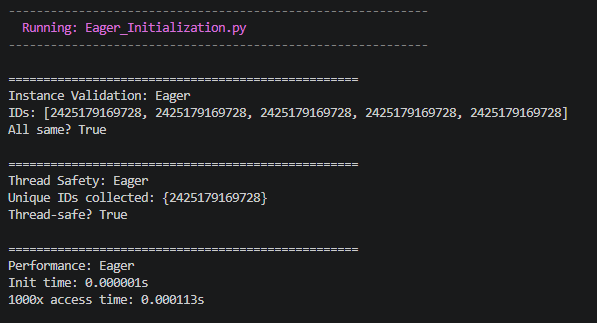
\includegraphics[width=0.95\textwidth]{eager.png}
    \caption{Eager Initialization: single instance ID in sequential and concurrent tests.}
\end{figure}

\begin{figure}[H]
    \centering
    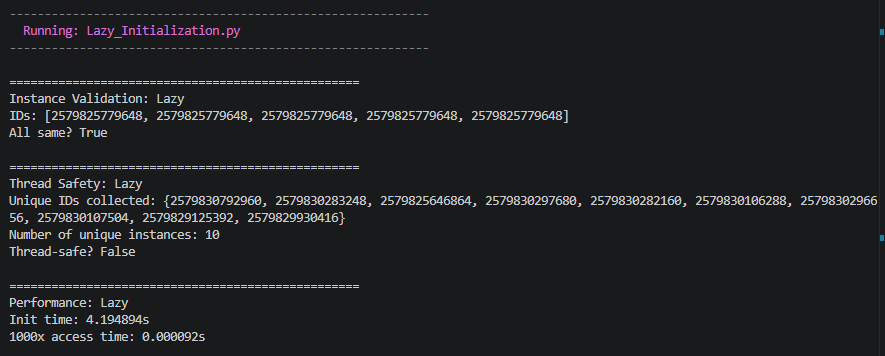
\includegraphics[width=0.95\textwidth]{lazy.png}
    \caption{Lazy Initialization: multithreaded run produced multiple instances (10 unique IDs).}
\end{figure}

\begin{figure}[H]
    \centering
    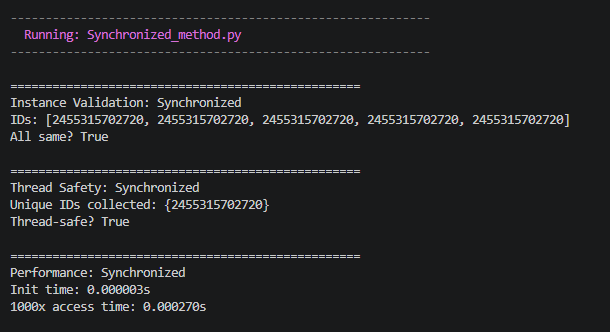
\includegraphics[width=0.95\textwidth]{syncronized.png}
    \caption{Synchronized Method: one instance maintained under concurrency.}
\end{figure}

\begin{figure}[H]
    \centering
    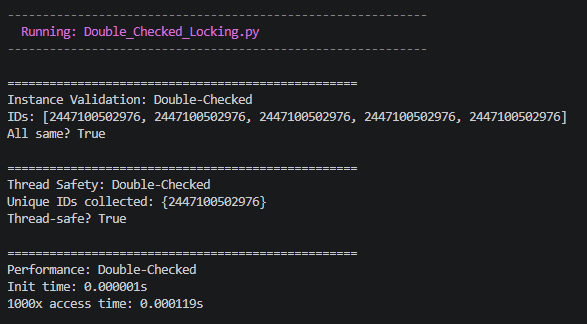
\includegraphics[width=0.95\textwidth]{double-checked.png}
    \caption{Double-Checked Locking: one instance maintained under concurrency.}
\end{figure}

\begin{figure}[H]
    \centering
    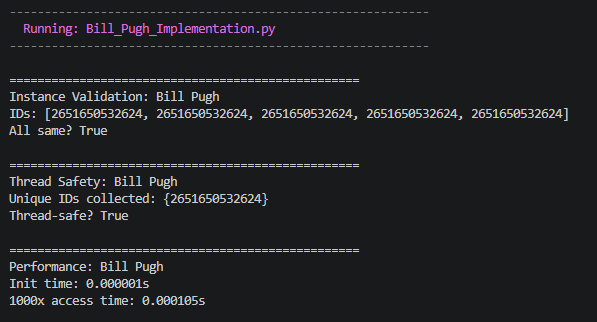
\includegraphics[width=0.95\textwidth]{bill-pugh.png}
    \caption{Bill Pugh: one instance maintained under concurrency.}
\end{figure}

\begin{figure}[H]
    \centering
    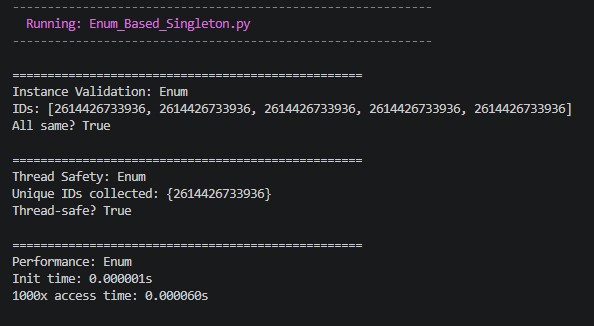
\includegraphics[width=0.95\textwidth]{enum.png}
    \caption{Enum-based Singleton: one instance maintained under concurrency.}
\end{figure}

\section{Performance Measurements}

\subsection*{Initialization Time}
Elapsed time for the first instance retrieval or creation in each implementation.

\subsection*{Access Time Under Repeated Calls}
Elapsed time for 1000 repeated instance access calls.

\begin{table}[H]
\centering
\caption{Performance comparison from observed output}
\begin{tabular}{@{} l S[table-format=1.6] S[table-format=1.6] @{}}
\toprule
Implementation & \multicolumn{1}{c}{Init time (s)} & \multicolumn{1}{c}{1000× access time (s)} \\
\midrule
Eager Initialization    & 0.000001 & 0.000113 \\
Lazy Initialization     & 4.194894 & 0.000092 \\
Synchronized Method     & 0.000003 & 0.000270 \\
Double-Checked Locking  & 0.000001 & 0.000119 \\
Bill Pugh Implementation& 0.000001 & 0.000105 \\
Enum-based Singleton    & 0.000001 & 0.000060 \\
\bottomrule
\end{tabular}
\end{table}

\subsection*{Observed Ranking by 1000× Access Time (Fastest to Slowest)}
\begin{enumerate}
    \item Enum-based Singleton (0.000060 s)
    \item Lazy Initialization (0.000092 s)
    \item Bill Pugh Implementation (0.000105 s)
    \item Eager Initialization (0.000113 s)
    \item Double-Checked Locking (0.000119 s)
    \item Synchronized Method (0.000270 s)
\end{enumerate}

\section{Comparative Summary (Based on Results Only)}

\subsection*{Which Implementations Are Fastest}
From observed 1000× access times, Enum-based Singleton is fastest (0.000060 s), followed by Lazy (0.000092 s) and Bill Pugh (0.000105 s).

\subsection*{Which Are Thread-Safe in Practice}
Eager Initialization, Synchronized Method, Double-Checked Locking, Bill Pugh, and Enum-based Singleton each produced exactly one unique instance under concurrent execution.

\subsection*{Which Show Inconsistencies}
Basic Lazy Initialization is inconsistent under concurrency: it produced 10 unique instances in the multithreading experiment, thus fails practical thread-safety.

\end{document}